\begin{figure*}

\raisebox{0.95cm}{%
  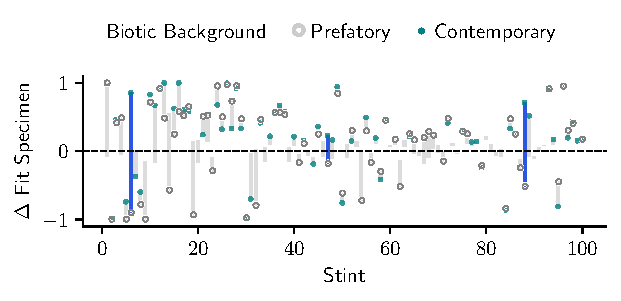
\includegraphics[
    width=0.51\linewidth,
    trim=0 1.1cm 0 0cm,
    clip
  ]{%
binder-2025-08-24-keyfig/binder/teeplots/2025-08-24-keyfig/baseline=prefatory+bbg=contemporary+dmaint=+subject=specimen+viz=signchangedotplot+ext=.pdf}%
}
%
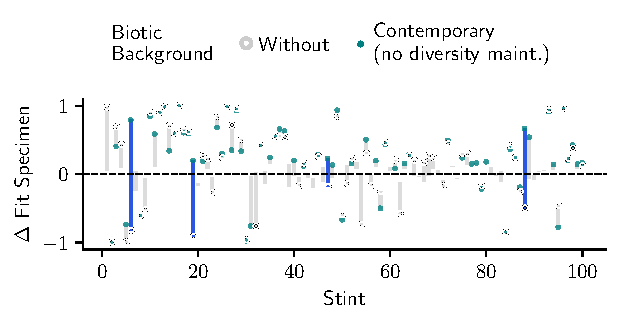
\includegraphics[width=0.45\linewidth,trim={1.2cm 0 0 0},clip]{%
binder-2025-08-24-keyfig/binder/teeplots/2025-08-24-keyfig/baseline=prefatory-no-diversity-maint+bbg=contemporary-no-diversity-maint+dmaint=no-diversity-maint+subject=specimen+viz=signchangedotplot+ext=.pdf}

\vspace{-6ex}

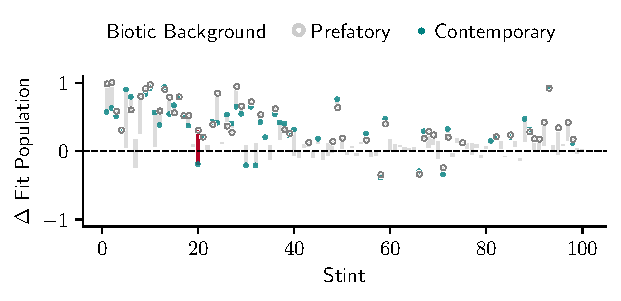
\includegraphics[width=0.51\linewidth,trim={0 0 0 1cm},clip]{%
binder-2025-08-24-keyfig/binder/teeplots/2025-08-24-keyfig/baseline=prefatory+bbg=contemporary+dmaint=+subject=population+viz=signchangedotplot+ext=.pdf}

\vspace{-1ex}

\caption{
\textbf{Fitness trade-offs between prefatory and contemporary ecological context.}
\footnotesize
Plots report influence on focal strain competition assays attributable to source of background strain used for ecological context.
Experiments competed focal strain samples (specimen or population from stint $n+1$ against baseline focal strain population from stint $n$.
Outcomes recorded between $1$ (fitness gain; stint $n$ baseline driven extinct) and $-1$ (fitness loss; stint $n+1$ driven extinct), with near-zero values indicating comparable fitness.
Under prefatory context, background strain from stint $n$; under contemporary context, stint $n+1$.
Vertical line segments mark discrepancy between conditions with prefatory background strain (i.e., from stint $n$; hollow markers) and contemporary background strain (i.e., from stint $n+1$; filled markers).
Markers omitted where no significant significant fitness change detected between stint $n+1$ and stint $n$ baseline ($\alpha = 0.005$).
Segment color highlights sign-change effect: harmful trait becomes beneficial with contemporary strain (blue) or vice versa (red).
Subplots differ in focal strain sample type (rows) and whether background-strain balancing diversity maintenance mechanism was enabled (columns).
Note that no assays with background strain diversity maintenance mechanism disabled were conducted for population-subject trials, owing to the lack of effect seen in specimen-subject trials (Supplementary Figure \ref{fig:sign-change-nodmaint-vs-nodmaint}).
}
\label{fig:sign-change-prefatory-vs-contemporary}

\end{figure*}
